%%
%% Copyright 2007-2020 Elsevier Ltd
%%
%% This file is part of the 'Elsarticle Bundle'.
%% ---------------------------------------------
%%
%% It may be distributed under the conditions of the LaTeX Project Public
%% License, either version 1.2 of this license or (at your option) any
%% later version.  The latest version of this license is in
%%    http://www.latex-project.org/lppl.txt
%% and version 1.2 or later is part of all distributions of LaTeX
%% version 1999/12/01 or later.
%%
%% The list of all files belonging to the 'Elsarticle Bundle' is
%% given in the file `manifest.txt'.
%%

%% Template article for Elsevier's document class `elsarticle'
%% with numbered style bibliographic references
%% SP 2008/03/01
%%
%%
%%
%% $Id: elsarticle-template-num.tex 190 2020-11-23 11:12:32Z rishi $
%%
%%
\documentclass[preprint,12pt]{elsarticle}

%% Use the option review to obtain double line spacing
%% \documentclass[authoryear,preprint,review,12pt]{elsarticle}

%% Use the options 1p,twocolumn; 3p; 3p,twocolumn; 5p; or 5p,twocolumn
%% for a journal layout:
%% \documentclass[final,1p,times]{elsarticle}
%% \documentclass[final,1p,times,twocolumn]{elsarticle}
%% \documentclass[final,3p,times]{elsarticle}
%% \documentclass[final,3p,times,twocolumn]{elsarticle}
%% \documentclass[final,5p,times]{elsarticle}
%% \documentclass[final,5p,times,twocolumn]{elsarticle}

%% For including figures, graphicx.sty has been loaded in
%% elsarticle.cls. If you prefer to use the old commands
%% please give \usepackage{epsfig}

%% The amssymb package provides various useful mathematical symbols
\usepackage{amssymb}
%% The amsthm package provides extended theorem environments
%% \usepackage{amsthm}
\usepackage{graphicx}
%\usepackage{caption}
\usepackage{comment}
\usepackage{amsmath}
\usepackage{subfigure}
\usepackage{booktabs}
\usepackage{float}
%\usepackage{pgfplots}
\usepackage{graphicx}
\usepackage{fullpage} % for full page width
\usepackage{lipsum} % for dummy text
\usepackage{adjustbox} % for adjusting graphics
\usepackage{xcolor}
\usepackage{hyperref}
\hypersetup{
     colorlinks=true,
     linkcolor=black,
     citecolor=black,
     filecolor=black,
     urlcolor=black,
 }

%% The lineno packages adds line numbers. Start line numbering with
%% \begin{linenumbers}, end it with \end{linenumbers}. Or switch it on
%% for the whole article with \linenumbers.
%% \usepackage{lineno}

\journal{Computer Methods in Applied Mechanics and Engineering}

\begin{document}

\begin{frontmatter}

%% Title, authors and addresses

%% use the tnoteref command within \title for footnotes;
%% use the tnotetext command for theassociated footnote;
%% use the fnref command within \author or \address for footnotes;
%% use the fntext command for theassociated footnote;
%% use the corref command within \author for corresponding author footnotes;
%% use the cortext command for theassociated footnote;
%% use the ead command for the email address,
%% and the form \ead[url] for the home page:
%% \title{Title\tnoteref{label1}}
%% \tnotetext[label1]{}
%% \author{Name\corref{cor1}\fnref{label2}}
%% \ead{email address}
%% \ead[url]{home page}
%% \fntext[label2]{}
%% \cortext[cor1]{}
%% \affiliation{organization={},
%%             addressline={},
%%             city={},
%%             postcode={},
%%             state={},
%%             country={}}
%% \fntext[label3]{}

\title{Enhancing Fractographic Fatigue Failure Analysis, Automated Flow Stress, and Fracture Toughness Evaluation in Fatigue Specimens - a Smart Approach with Artificial Intelligence and Image Processing}

%% use optional labels to link authors explicitly to addresses:
%% \author[label1,label2]{}
%% \affiliation[label1]{organization={},
%%             addressline={},
%%             city={},
%%             postcode={},
%%             state={},
%%             country={}}
%%
%% \affiliation[label2]{organization={},
%%             addressline={},
%%             city={},
%%             postcode={},
%%             state={},
%%             country={}}
\author[Computer_b]{Or Haim Anidjar}
\author[Computer_a]{Jonatan Boritski}
\author[Computer_a]{Avichay Mazin}
\author[Computer_a]{Sapir Dahan}
\author[Afeka]{Oz Golan}
\author[soreq]{Elad Farkash}
\author[fracture]{Mor Mega}
%\author[Computer_a,Computer_a,Computer_b]{Avichay Mazin$^a$, Jonatan Boritski$^a$, Or Anijar$^b$, Sapir Dahan$^a$, Elad Farkash$^c$, Mor Mega$^d$}

\affiliation[Computer_a]{organization={Department of Computer Science, \\Ariel University},%Department and Organization
            city={Ariel},
            postcode={40700},
            country={Israel}}

\affiliation[Computer_b]{organization={Department of Computer Science, \\Ariel University},%Department and Organization
            city={Ariel},
            postcode={40700},
            country={Israel}}

\affiliation[soreq]{organization={Soreq Nuclear Research Center},%Department and Organization
            city={Yavne},
            postcode={81800},
            country={Israel}}

\affiliation[fracture]{organization={The Fracture and Fatigue Research Laboratory, \\Department of Mechanical Engineering and Mechatronics, \\Ariel University},%Department and Organization
            city={Ariel},
            postcode={40700},
            country={Israel}}

\affiliation[technion]{organization={Faculty of Mechanical Engineering, Technion - Israel Institute of Technology},%Department and Organization
city={Haifa},
postcode={32000},
country={Israel}}

\begin{abstract}
%% Text of abstract

\end{abstract}

%%Graphical abstract
\begin{graphicalabstract}
%\includegraphics{grabs}
\end{graphicalabstract}

%%Research highlights
\begin{highlights}
\item Research highlight 1
\item Research highlight 2
\end{highlights}

\begin{keyword}
%% keywords here, in the form: keyword \sep keyword

%% PACS codes here, in the form: \PACS code \sep code

%% MSC codes here, in the form: \MSC code \sep code
%% or \MSC[2008] code \sep code (2000 is the default)

\end{keyword}

\end{frontmatter}

%% \linenumbers

%% main text
\section{Introduction}
\label{Sec:Introduction}


\begin{comment}
\subsection{Today Scene: What We Have and What Might Evolve}  \label{Subsec:Today's Scene: What We Have and What Might Evolve}
The application of machine learning and deep learning for analyzing fracture surfaces and extracting meaningful information has seen a significant rise in the last years as discussed in a study \cite{tsopanidis2020unsupervised}.
As we can see in the article, these tools are not only facilitate the extraction of valuable insights that may surpass the capabilities of traditional fractographic experts, but also introduce automation, making the entire process more efficient and time saving.

In practical terms, utilizing machine and deep learning for fracture surface analysis proves to be a time saving effort. Instead of the manual analysis of fracture surfaces, which can be time consuming, these advanced tools simplify the process. Moreover, the accuracy and effectiveness of the analyses are often hig enough that, in certain cases, reliance on traditional fractographic experts may become unnecessary. The automated nature of machine and deep learning analyses contributes to a more efficient, rapid, and sometimes even superior understanding of fracture surfaces.
\par
As we explain earlier, an analysis of fatigue failure in engineering structures has already been done before in some aspects.
For example, in previous studies, some researchers have already made an analysis about fractions materials produced through 3D printing. One is the research \cite{anidjar2023transfer}.
 This research emphasize why is important to analyze fractures in materials and explain that fractographic analysis plays a crucial role in understanding the mechanical properties and fatigue behavior of materials, especially in identifying the primary causes of failure. For this problem, the challenge of identifying fatigue crack initiation sites, the researchers attitude towards the solution for the problem was innovation and efficiency. They recognized that the process of identifying and characterizing fatigue crack initiation sites in materials can be time consuming and costly when done manually. Therefore, they try to develop a computer vision based approach that could automate and expedite the process.
the researchers have been used in two deep learning algorithms. One is called ResNet152 and it used to filter out image sections that do not contain the fatigue crack initiation site. The second is called YOLOv5 which used for object detection. After the irrelevant image sections have been filtered out by ResNet152, YOLOv5 is trained to detect and classify the remaining image sections to precisely identify the initiation site.
\end{comment}



%\subsection{Mechanical Background}
\textcolor{green}{
Additive Manufacturing (AM) technology, also known as 3D printing, is an innovative process wherein parts are fabricated layer by layer, adhering to three-dimensional digital models. This innovative technique, emerged in the late 1980s, has made a significant advancement in manufacturing technology. Widely referred as a cornerstone of the third industrial revolution, AM offers almost unlimited opportunities for the creation of intricately designed products, which is markedly different from traditional metal manufacturing methods~\cite{wong2012review}. One of the biggest advantages of AM lies in its obviation of the need for molds, a factor that substantially diminishes production costs and enables the production of complex components~\cite{herzog2016additive}.}

\subsection{Titanium Alloys in Additive Manufacturing}

\textcolor{green}{
Titanium alloys are highly advanced structural materials known for their diverse set of exceptional properties. These include resistance to corrosion in seawater, impressive strength-to-weight ratios, excellent fracture toughness, high fatigue resistance, strong compatibility with composites, long-term durability with minimal maintenance requirements, and exceptional biocompatibility~\cite{qian2016additive}. Despite the extensive exploration of the static mechanical properties of AM materials, encompassing factors such as strength, stiffness, and impact energy~\cite{debroy2018additive,gorsse2017additive}, investigations into their dynamic performance and fatigue characteristics remain comparatively scant. Additive Ti-6Al-4V is increasingly esteemed as promising lightweight structural components in aerospace and automotive sectors~\cite{boyer1996overview,debroy2018additive}. In these areas, the ability to withstand fatigue loads is critical. However, a comprehensive understanding of its fatigue behavior and underlying failure mechanisms remains elusive. Hence, delving into the mechanical fatigue properties of AM materials becomes imperative.}

\subsection{Traditional and Additive Manufacturing Methods}
\textcolor{green}{One of the traditional methods for manufacturing Ti-6Al-4V alloys is subtractive manufacturing (SM), where material is machined away from a solid block to achieve the desired shape. This approach is inherently inefficient and resource-intensive. According to~\cite{peng2017toward}, an excessive portion of the material is removed and discarded during the process, resulting in increased costs and significant waste, contributing to notable ecological impacts.
In contrast, advanced manufacturing techniques such as Selective Laser Melting (SLM) allow producing near-net-shape components from CAD models by producing parts layer by layer, significantly reducing material waste and time consumption, as shown in~\cite{fatimah2013sustainable}. This method is particularly advantageous for producing complex geometries, as it eliminates the need for molds and tooling, as shown in~\cite{huang2016energy}, especially in the context of lightweight aircraft components.
Electron Beam Melting (EBM) is another additive manufacturing (AM) technique that, like Selective Laser Melting (SLM), melts metal powder layer by layer to fabricate solid objects.
However, EBM operates on a much wider scale compared to SLM.}

\subsection{Challenges in Additive Manufacturing}
\textcolor{green}{

The SLM process has intrinsic limitations, such as the formation of uncontrolled defects, including porosity, cracks, and inclusions, which can significantly impair the mechanical properties of the final product. The shift in the field of fracture mechanics from evaluating static material properties such as strength and toughness to analyzing dynamic properties like fatigue and fracture behavior has been a significant development. This shift is crucial for understanding the material's performance under dynamic loading conditions, such as heat, pressure, vibration, and cyclic loading.}


\subsection{Fatigue Characterisitcs of Additive Manufactured Alloys}

\textcolor{green}{Fatigue failure of engineering components and structures results from progressive fracture caused by cyclic or fluctuating loads. Fatigue is an important potential cause of mechanical failure because most engineering components or structures can be subjected to cyclic loads during their lifetime.
An abbreviated summary of fatigue processes and mechanisms: fatigue crack initiation, propagation, and final fracture. Characteristic fatigue fracture features that can be visually discerned under low magnification are then described.
Typical microscopic features observed on structural metals are presented.}

\textcolor{green}{
The flow stress and stress intensity factor are critical parameters for predicting the final failure of a specimen under cyclic fatigue loading. The flow stress parameter, \(\sigma_{\text{net}}\), is related to the applied force and the uncracked area of the specimen. When \(\sigma_{\text{net}}\) reaches the failure stress, \(\sigma_f\), the specimen fails, and crack initiation occurs. The stress intensity factor, \(K_I\), is linked to the fracture toughness, \(K_{IC}\), of the material. When \(K_I\) reaches \(K_{IC}\), crack propagation occurs. Once the crack reaches the critical size, the specimen fractures completely. Understanding \(\sigma_{\text{net}}\) and \(K_I\) is crucial for predicting material failure, designing safe structures, and selecting appropriate materials. These parameters illustrate internal resistance and stress concentration around cracks, thereby preventing catastrophic failures and enhancing material robustness.}
\textcolor{green}{
Fatigue crack propagation can be divided into three stages: initiation, propagation, and final fracture. In Stage I, the initiation stage, cracks propagate along high shear stress planes (45 degrees) with microstructural barriers like grain boundaries decelerating the process. Surface treatments such as shot peening and surface rolling increase the number of microstructural barriers, helping to prevent fatigue cracks. Stage II begins with an increase in the stress intensity factor, \(K\), which predicts the stress state near the crack tip due to remote load or residual stresses. The value of \(K\) depends on sample geometry, crack size and location, and load distribution. As \(K\) increases from crack growth or higher applied loads, slips develop near the crack tip. Stage III is the unstable part of crack growth, occurring when \(K_{\text{max}}\) approaches \(K_{IC}\). This leads to rapid material failure due to cyclic static mode failures, with significant sensitivity to microstructure, load ratio, and stress state. The instability of Stage III limits the information extractable from its surface \cite{newman1981empirical}.}

\begin{comment}
    In \textcolor{red}{need more up to date papers if these are examples for papers that made use of the method we are using... If not, then examples of what are these?}~\cite{astiz1986incompatible,carpinteri1992stress,carpinteri1992elliptical}, models for predicting the stress intensity factor for such a geometry were proposed.

\textcolor{green}{Additive Manufacturing\\Fatigue\\Fractografic analysis and surface regions\\stress intensity factor calculation models\\flow stress calculation models\\It may be useful to solve this using computer vision methods  (no equations, just references)}
\end{comment}

\subsection{Computer Vision and Machine Learning in Additive Manufacturing}
\textcolor{green}{

Computer vision and machine learning techniques have been increasingly employed in the field of additive manufacturing to address challenges related to material characterization, defect detection, and failure analysis. During the additive manufacturing (AM) process, materials may experience changes in their properties, potentially leading to failures and defects. To address these challenges, researchers typically investigate the process in three chronological stages:

\begin{enumerate}
    \item \textbf{Preprocessing} - Gathering and analyzing material characteristics before the AM process begins. In ~\cite{miyazaki2019image}, the authors conducted a study on the influence of heat treatment during the SLM process on the micro-structure and mechanical properties of Ti-6Al-4V. They utilized machine learning techniques for image segmentation and analysis.
    \item \textbf{In-Process Monitoring} - Monitoring in additive manufacturing involves using various sensors to collect real-time data on production tasks, including indicators, signals, and images, to detect defects and ensure process control. Laser welding is an additive manufacturing process commonly used for materials welding, especially in the automated welding of small components, within sectors such as medical devices, aerospace components, and electronics. In~\cite{cai2023real}, an CNN model was developed, along with an adaptive fusion image method to eliminate some of the noise in the images, to monitor the penetration state during laser keyhole welding, ensuring the quality of the welding process.
    \item \textbf{Postprocessing} - Evaluating and analyzing the material after the AM process is completed. Applying ML techniques to achieve accurate classification and segmentation of defects, similar to the method used by Dung et al. who constructed a deep FCN with VGG16 as the backbone to achieve crack detection by means of semantic segmentation of concrete images \cite{pu2022autonomous}.
\end{enumerate}

This study specifically focuses on the post-processing stage, aiming to characterize the Ti-6Al-4V alloy by evaluating its stress intensity factor and flow stress after the AM process.}


\subsection{Related Work}  \label{Subsec:Related Work}
    The integration of computer vision in the field of fracture mechanics, particularly in the analysis of metal fractures, has evolved significantly over recent years.
    In its early stages, the approach primarily relied on Scanning Electron Microscope (SEM) images and conducting manual classification efforts.
    However, the traditional process is manual, labor-intensive, and prone to human error.
    Automating this process and developing quantitative methods for studying fracture surfaces is a major challenge but has significant industrial and scientific potential.
    Automated fractography could enhance the reliability of failure analysis and uncover new insights into material failure mechanisms.




    Early applications in fracture mechanics prioritized image processing over the more advanced computer vision and machine learning techniques.
    These initial approaches were designed to enhance features in images of fracture surfaces captured by SEM and optical microscopy, with a greater emphasis on qualitative rather than quantitative analysis.
    Fundamental techniques employed in these efforts included spatial domain methods like texture analysis and the Gray Level Co-occurrence Matrix (GLCM) for fractal analysis.
  In \cite{zain2009enhancement}, the authors experimented with various spatial filtering techniques such as mean, median, Gaussian, and Wiener filters to enhance the quality of the identification of the fracture image.
    In the engineering field, another set of experiments can be observed In \cite{das2011characterization}, where the changes on the surface are effectively characterized using these methods.
    Furthermore, some of these techniques also incorporated transform domain methods, such as Fourier transform, wavelet transform, and Gabor transform.
    In another study, In \cite{hu2017automation}, the authors employed edge detection and peak-finding algorithms to determine the progression marks associated with fatigue crack growth.

    These methods were applied to optical and Scanning Electron Microscopy (SEM) images to classify and characterize fracture surfaces.
    However, these methods often required additional user input and assumptions, which limited their robustness and applicability, especially for complex surfaces.

    Recent developments have seen the use of machine learning and artificial intelligence in materials characterization, including micro-structure classification and defect analysis.
    Promising machine learning methods like artificial neural networks and support vector machines have played a pivotal role in classifying observed fractures, yielding promising results in materials characterization.
    Some notable achievements in this area include the use of a complex CNN architecture known as Unet,
    as demonstrated In \cite{tsopanidis2020toward}, where an accuracy of 71.2 percent in Intersection over Union (IOU) was achieved for triple-class classification,
    distinguishing inter-granular and trans-granular fracture events from scanning electron microscope images.
    Another article compared a more intricate Unet neural network architecture, reaching an accuracy of 86 percent in the Dice score accuracy metric for the segmentation task of detecting dimple fractures \cite{sinha2021deep}.

    A prominent trend has emerged in recent times where a fusion of traditional image processing methods and cutting-edge AI techniques has been observed.
    In these approaches, a pivotal role is played by feature extraction during the prepossessing phase, enhancing the salient characteristics within images.
    As exemplified \textcolor{red}{In \cite{naik2019identification}}, researchers combined texture recognition algorithms, specifically the Local Binary Pattern (LBP), with the classical machine algorithm called Linear Discriminant Analysis (LDA). This innovative combination allowed them to identify the fracture type and its area in both brittle and ductile materials by leveraging the uniqueness of texture features, achieving an impressive accuracy rate of 94 percent.
    Another notable example is presented \textcolor{red}{In \cite{bastidas2016fractographic}}, where SVM classification was employed to classify three different types of fractures in crystalline materials.

       In the field of fracture mechanics, certain techniques leverage the connection between computer vision and machine learning for fracture surface analysis. Feature extraction methods, such as edge detection using the Sobel operator, can enhance image quality and denoise the image, isolating the necessary features and improving the accuracy of models. For instance, Wang et al. (2019) introduced an improved Sobel operator combined with Otsu thresholding for feature extraction in the classification of cracks in concrete bridge structures \cite{wang2019research}. This method utilized image vertical and horizontal projection profiles to classify four types of cracks.
    Inspired by this enhancement method, a comparative analysis was conducted to assess the performance of these contrast enhancement methods along with a Deep Convolution Neural Network (DCNN) for a binary classification task. This approach achieved a 16.8\% improvement in accuracy over images without enhancement, as demonstrated by Bhalaji et al. (2024) \cite{bhalaji2024transfer}.

    An advancement in this research lies in the integration of the localization problem with the feature extraction phase.
    As demonstrated \textcolor{red}{In \cite{zhang2023automated}}, a remarkable achievement was reached with a detection rate of up to 92 percent in terms of the F1 score for detecting bridge cracks.
    This approach was developed by segmenting the process into three distinct phases: initially selecting specific regions, then extracting features using methods like SIFT and HOG, and finally applying the YOLO neural network architecture for precise object localization and detection.


In this study, an innovative approach is proposed to automate the analysis of fatigue fracture surfaces in Ti-6Al-4V specimens produced through additive manufacturing.
The approach utilizes a multi-stage process, including image preprocessing, feature extraction, and classification.
Image preprocessing involves removing extraneous metadata and resizing images to a uniform resolution, ensuring that the learning algorithms focus solely on the relevant features of the specimens.
Feature extraction is achieved through the calculation of the magnitude of gradients over the images to produce heat-map using a Sobel transform, which enhances the images for easier analysis and enables the identification of fatigue crack propagation areas.
The classification phase involves the use of a specialized neural network architecture known as UNet, renowned for its efficacy in image segmentation task.
This network is utilized to identify and classify the contours of fatigue crack propagation areas using heatmap images generated in the previous stage, alongside the overall specimen contour on the original image.
Finally, computer vision techniques are employed to detect the elliptical crack front to calculate both the stress intensity factor and the flow stress of the specimen, based on the detected contours.





\section{Terms and Definitions}

\subsection{Mechanical basic terms}  \label{sec:Basic terms}


Two failure criteria may be used to predict the final failure of a specimen subjected to cyclic fatigue loading. The first criterion is related to the flow stress parameter \(\sigma_{net}\), and the second is related to the stress intensity factor \(K_{I}\). Once one of these parameters reaches a critical value, failure is expected. The model used here to determine the flow stress in a bar specimen tested in cyclic fatigue is presented in Section~\ref{Subsec: Flow stress calculation model}.
In Section~\ref{Subsec: Stress intensity factors calculation model}, several closed-form solutions for the determination of \(K_I\) are introduced and the best one is chosen \cite{shin2004experimental}.


\subsubsection{Fractographic image analysis description}
\label{Subsec: Fractographic image analysis}

\subsubsection{Flow stress calculation model}
\label{Subsec: Flow stress calculation model}
\begin{figure*}[t!]
  \begin{center}
  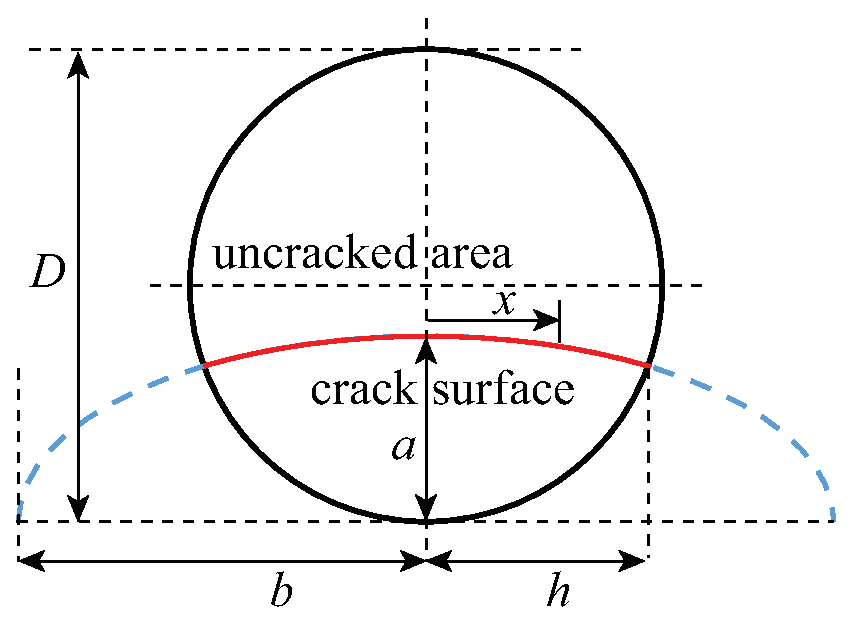
\includegraphics[width=3in]{elliptical_surface_crack.eps}
  \caption{Schematic view of an elliptical crack.}
  \label{fig:elliptical_crack}
   \end{center}
\end{figure*}

One known failure criterion is based on the calculated flow stress $\sigma_{net}$. Once this parameter reaches the failure stress $\sigma_{f}$, the final failure will occur.

The failure stress \(\sigma_{f}\) is related to the ligament area, defined as the uncracked area illustrated in Fig.~\ref{fig:elliptical_crack}. For a specific material, the value of \(\sigma_{f}\) is given by \cite{kanchanomai2004low}
%
\begin{equation}
    \sigma_{f} = \frac{\sigma_Y + \sigma_{UTS}}{2}
\end{equation}
%
where \(\sigma_Y\) is the yield stress and \(\sigma_{UTS}\) is the ultimate stress of the material.

The flow stress, \(\sigma_{net}\), is a function of the applied force and the uncracked area, namely,
%
\begin{equation}
\label{eq:sig_net}
\sigma_{net}= \displaystyle\frac{\sigma_{max} A_0}{A_{\textit{uncracked area}}}
\end{equation}
%
where $\sigma_{max}$ is the maximum applied stress in each fatigue cycle, \(A_0\) is the total area of the specimen surface, and \(A_{\text{uncracked area}}\) is the ligament area illustrated in Fig.~\ref{fig:elliptical_crack}. Once \(\sigma_{net}\) reaches the value of \(\sigma_f\), the specimen will fail.
%
%

\subsubsection{Stress intensity factor calculation model}
\label{Subsec: Stress intensity factor calculation model}
%
%
\begin{table}[t!]
\caption{Tabulated values of $M_{i,j,k}$ in eq.~(\ref{eq:F_I}). \strut}
\label{tab:M_ijk}      % Give a unique label
\resizebox{\columnwidth}{!}{
\begin{tabular}{cccclccclccc}
\noalign{\bigskip}\hline\noalign{\smallskip}\hline
  &          & k=0       &           &  &          & k=1       &          &  &         & k=2      &           \\ \cline{2-4} \cline{6-8} \cline{10-12}
j & i=0      & 1         & 2         &  & i=0      & 1         & 2        &  & i=0     & 1        & 2         \\
0 & 1.095    & -1.177    & 0.725     &  & 0.113    & 0.271     & -0.388   &  & -0.896  & 0.904    & 0.008     \\
1 & -1.336   & 17.924    & -17.427   &  & 1.824    & -11.649   & 10.074   &  & 3.092   & 0.701    & -4.883    \\
2 & 13.108   & -137.252  & 134.652   &  & -21.709  & 98.358    & -80.088  &  & -4.197  & -32.641  & 55.092    \\
3 & -43.689  & 545.816   & -551.902  &  & 105.483  & -415.027  & 328.165  &  & -13.255 & 204.104  & -305.079  \\
4 & 134.868  & -1223.334 & 1239.493  &  & -271.225 & 982.713   & -772.921 &  & 51.548  & -568.407 & 916.962   \\
5 & -242.653 & 1541.587  & -1548.537 &  & 387.47   & -1329.634 & 1055.952 &  & -59.329 & 857.543  & -1545.428 \\
6 & 254.093  & -1006.656 & 969.388   &  & -290.024 & 961.893   & -784.581 &  & 13.481  & -657.659 & 1372.595  \\
7 & -108.196 & 264.206   & -227.132  &  & 88.387   & -288.565  & 245.798  &  & 10.854  & 191.57   & -485.556  \\
\hline\noalign{\smallskip}\hline
\end{tabular}
}
\end{table}
An additional known failure criterion is based on the stress intensity factor $K_I$ value. Once this parameter reaches the fracture toughness $K_{Ic}$ of the tested material, the crack will propagate, and final failure will occur. The critical stress intensity factor or fracture toughness value \(K_{Ic}\) is reached once the crack approaches a critical size.



In~\cite{toribio2009automated}, it was demonstrated that the crack front in a fatigue bar specimen may be treated as an ellipse with the center located at the specimen surface, as illustrated in Fig.~\ref{fig:elliptical_crack}. The parameters $a$ and $b$ are the major and minor diameters of the ellipse in Fig.~\ref{fig:elliptical_crack}, respectively. These dimensions represent the depth and width of the crack, respectively. The parameter $D$ is the total specimen diameter, $x$ is a chosen coordinate between 0 and $h$ where $h$ is the horizontal distance between the center of the ellipse and the intersection between the ellipse and the specimen outer surface. It may be noted that the axis of symmetry of the ellipse is the same as the axis of symmetry of the bar and the center of the ellipse is on the edge of the rod. All parameters are shown in Fig.~\ref{fig:elliptical_crack} and may be used to calculate $K_I$.

Next, several closed-form solutions are presented and the best one is chosen. In~\cite{valiente1980criterios}, the first closed-form solution was introduced. This form was only for a straight front crack ($b$ limit to infinity). The value of $K_I$ is calculated only at the center of the crack front.
In~\cite{astiz1986incompatible}, a closed-form solution is introduced for an elliptical crack front; but $K_I$ is found only in the center of the crack front. In~\cite{couroneau1998simplified,carpinteri1992elliptical} two closed-form solutions were presented, one at the crack front center, shown as point A in Fig.~\ref{fig:elliptical_crack}, and another for the end of the crack front, shown as point G in Fig.~\ref{fig:elliptical_crack}. In \cite{shin2004experimental} a closed-form solution was found based on the FE method and the virtual crack extension technique~\cite{hellen1975method}. The solution was found as a function of $a$, $b$, and $x/h$ the location along the crack front, as shown in Fig.~\ref{fig:elliptical_crack}.
Another solution that uses these three parameters~\cite{shih2002stress} was found to produce negative results. A detailed review of these solutions and other solutions may be found in~\cite{toribio2009automated}.
It was found~\cite{toribio2009automated} that the best closed-form solution for the problem in this research is~\cite{shih2002stress}.


In~\cite{shin2004experimental}, the closed-form solution is based on the FE method and the virtual crack extension technique~\cite{hellen1975method}.  The calculation of \(K_I\) is proposed as
%
\begin{equation}
\label{eq:K_I__F_I}
K_{I}=F_I \sigma_0 \sqrt{\pi a}
\end{equation}
%
where $F_I$ is a function of $a, b, D, h$ and $x$ given as
%
\begin{equation}
\label{eq:F_I}
F_{I}=\sum^{2}_{i=0} \sum^{7}_{j=0}\sum^{2}_{k=0} M_{ijk}\left(\frac{a}{b}\right)^i  \left(\frac{a}{D}\right)^j  \left(\frac{x}{h}\right)^k\;\;.
\end{equation}
In eq.~(\ref{eq:F_I}) the coefficients $M_{ijk}$ were determined from FEAs in \cite{shin2004experimental} and presented in Table~\ref{tab:M_ijk}.






\section{Neural Network Terms}
\label{sec:network_terms}

\subsection{Introduction to Neural Networks}

\textcolor{green}{Neural networks are advanced computational models inspired by the human brain's neural structure. They consist of interconnected units called neurons, organized into layers: the input layer (which receives the data), hidden layers (which process the data), and the output layer (which produces the final output). Each connection between neurons has an associated weight and bias, which are adjusted during training to minimize the error in the network's predictions \cite{lecun2015deep}.}

The learning process of a neural network involves several key steps:

\begin{enumerate}
    \item \textbf{Forward Pass:} Input data is passed through the network, layer by layer, to generate predictions. Each neuron performs a weighted sum of its inputs and passes the result through an activation function to introduce non-linearity.
    \item \textbf{Error Calculation:} The difference between the predicted output and the actual output (the error) is calculated using a loss function. Common loss functions include Mean Squared Error (MSE) for regression tasks and Cross-Entropy Loss for classification tasks \cite{goodfellow2016deep}.
    \item \textbf{Backward Pass (Backpropagation):} The error is propagated backward through the network. The gradients of the loss function with respect to each weight are computed using the chain rule of calculus. These gradients indicate how much each weight contributes to the overall error \cite{rumelhart1986learning}.
    \item \textbf{Weight Update:} The weights and biases are updated using an optimization algorithm, such as Stochastic Gradient Descent (SGD) or Adam, to reduce the error. This process iterates until the network's predictions are sufficiently accurate \cite{kingma2014adam}.
\end{enumerate}

Optimization algorithms like Adam further enhance the training process by adapting the learning rate for each parameter, making the training more efficient and effective \cite{kingma2014adam}.

Neural networks have demonstrated remarkable performance in various tasks. For instance, in image recognition, neural networks can learn to identify and classify objects within images with high accuracy, as evidenced by the success of deep residual networks \cite{he2016deep}. Similarly, in natural language processing, neural networks have enabled significant advancements in understanding and generating human language, as showcased by the development of transformer models \cite{vaswani2017attention}. Furthermore, neural networks are pivotal in predictive analytics, where they uncover complex patterns and relationships within data, crucial for making accurate predictions \cite{schmidhuber2015deep}.

\subsection{Description of U-Net Architecture}

U-Net is a neural network architecture specifically designed for image segmentation tasks \cite{ronneberger2015u}. It is composed of two main parts: the contracting path and the expansive path, connected by skip connections.

\subsubsection{Contracting Path}

The contracting path functions like a standard convolutional neural network (CNN). It consists of repeated application of convolutional layers, each followed by a rectified linear unit (ReLU) activation function and a max pooling operation. The convolutional layers capture features such as edges and textures, while max pooling reduces the spatial dimensions of the image, preserving essential features. This path captures the context and down-samples the image to a lower resolution while increasing the number of feature channels.

\subsubsection{Expansive Path}

The expansive path rebuilds the image to its original resolution. It uses transposed convolutions (or upsampling) to increase the size of the feature maps. Each upsampling step is followed by a concatenation with the corresponding feature map from the contracting path via skip connections, ensuring that detailed information is preserved. The combined feature maps undergo additional convolutions to refine the segmentation \cite{ronneberger2015u}.

Skip connections play a crucial role by directly linking corresponding layers in the contracting and expansive paths. This direct connection helps retain fine-grained details that might otherwise be lost during downsampling, ensuring precise and detailed segmentations.

\begin{figure}[h!]
\centering
\includegraphics[width=1\textwidth]{figures/UNet.png}
\caption{Illustration of the U-Net architecture, showcasing the contracting path on the left side and the expansive path on the right side \cite{ronneberger2015u}.}
\label{fig:unet_architecture}
\end{figure}

\subsection{Image Segmentation and Evaluation Metrics}

Image segmentation is the process of dividing an image into distinct regions, often for the purpose of identifying and classifying objects within the image. U-Net is particularly effective for segmentation tasks due to its ability to capture context and detail simultaneously.

Evaluating the performance of image segmentation models is crucial. Common metrics include:

\begin{itemize}
    \item \textbf{Dice Coefficient:} This metric measures the overlap between the predicted segmentation and the ground truth. As seen in prior research, it is calculated as:
    \[
    \text{Dice} = \frac{2|X \cap Y|}{|X| + |Y|}
    \]
    where \(X\) is the predicted segmentation and \(Y\) is the ground truth. A higher Dice coefficient indicates better segmentation performance \cite{milletari2016v}.

    \item \textbf{Intersection over Union (IoU):} Also known as the Jaccard index, this metric compares the overlap between the predicted segmentation and the ground truth relative to their combined area. It is formulated as:
    \[
    \text{IoU} = \frac{|X \cap Y|}{|X \cup Y|}
    \]
    where \(X\) and \(Y\) are the predicted segmentation and the ground truth, respectively. Higher IoU values indicate more accurate segmentation \cite{rahman2016optimizing}.
\end{itemize}

These metrics help quantify how well the model's segmentation matches the true segmentation, providing a clear measure of accuracy.








\section{Dataset} \label{Sec:dataset}

\textcolor{green}{The dataset utilized in this research comprises 63 Scanning Electron Microscope (SEM) images of Ti-6Al-4V alloy fatigue specimens. Each image is captured at a resolution of 4576 by 4096 pixels, enabling detailed examination of the specimens over an area of 5.5 mm with a pixel size of approximately 1.34 $\mu$m, as such a fine resolution is crucial because it enables the observation of minute details and microstructural features, which are essential for understanding the material’s fatigue behavior at a microscopic level.
This is particularly important for subsequent analysis phases, including image preprocessing and computer vision feature extraction stages, where preserving all details without information loss is critical, and resolution manipulation is unnecessary.
The dataset is organized into three categories based on the print quality recommended by the manufacturer: 30 images in P1 for standard printing, 21 in P2 for enhanced quality, and 12 in P3 indicating lower quality. These groupings reflect different levels of manufacturing precision, which may be relevant for specific analyses.
This approach enriches the dataset with diverse specimens, enabling a comprehensive examination of fatigue fracture surfaces across various print qualities and facilitating a more nuanced understanding of the material's fatigue behavior under different conditions.
Detailed documentation on specimen production and experimental setups, as referenced in previous work \cite{navickaite2022efficient}, provides essential background for understanding the context of these SEM images.}


\begin{figure}[h!]
  \centering
  \includegraphics[width=0.8\textwidth]{figures/side_by_side.png}
  \caption{SEM images of a Ti-6Al-4V fatigue specimen from two opposing viewpoints (A and B), showcasing the fracture surfaces from the lower and upper surfaces at different angles.}
  \label{same_material_from_both_sides}
\end{figure}

\paragraph{Inclusion of Duplicated Images}
A significant feature of this dataset is the inclusion of duplicated images for certain specimens, which were captured from the upper and lower surfaces of the specimens at different angles. This duplication is instrumental in providing a more holistic examination of the material's structural integrity and failure mechanisms, enhancing the understanding of fatigue fracture surfaces, as well as enriching the dataset with a broader range of fracture patterns and features.  Figure~\ref{same_material_from_both_sides} illustrates this approach by displaying SEM images of a Ti-6Al-4V fatigue specimen from two contrasting viewpoints, labeled A and B, which showcase both the lower and upper surfaces at different angles, of an identical specimen.



\paragraph{Dataset Design for Machine Learning Analysis}
The dataset is meticulously structured to support machine learning endeavors, particularly for the identification and analysis of fracture patterns and material defects. The precise categorization and comprehensive documentation of the images are crucial for facilitating accurate algorithmic training and validation. These steps are fundamental in developing robust predictive models that can reliably forecast material failures.

This well-organized dataset serves not only the specific objectives of this research but also enhances the broader field of materials science. It offers valuable insights into the mechanical properties and failure mechanisms of aerospace materials, thereby contributing significant knowledge to the scientific community. Such contributions are vital for advancing understanding and technology in material durability and safety.



\vspace{\baselineskip}
\vspace{\baselineskip}
\vspace{\baselineskip}






\section{Proposed Artificial Intelligence-driven Framework}
\label{Sec: Proposed Artificial Intelligence-driven Framework}
\subsection{Preliminary Operations}
\label{subsec:preliminary_operations}

\textcolor{green}{The conversion of raw data into a format suitable for deep learning was conducted using TensorFlow, an esteemed open-source machine learning framework renowned for its robust capabilities in image processing and model development. This preliminary phase involved several critical steps to refine the dataset for comprehensive analysis with our specialized UNet models, thereby ensuring the accurate representation of material fracture complexities. }

TensorFlow provided a comprehensive suite of pre-built functions and methods which were instrumental in this process. The \texttt{tf.data.Dataset.from\_tensor\_slices} method was utilized to create a scalable and efficient input pipeline, facilitating the seamless handling of large datasets. For image preprocessing, the \texttt{tf.image.resize} function was employed to standardize the dimensions of the images, while \texttt{tf.image.convert\_image\_dtype} was used to normalize pixel values. Additionally, the \texttt{tf.keras.preprocessing.image.ImageDataGenerator} function enabled real-time data augmentation, significantly enhancing the diversity of the training dataset without necessitating additional manual annotations.

The selection of TensorFlow over other machine learning frameworks was driven by several distinct advantages. Firstly, TensorFlow’s integration with Keras provided a high-level interface that simplified the development and implementation of complex deep learning models. Secondly, TensorFlow's robust support for distributed computing facilitated the efficient training of models across multiple GPUs, thereby considerably reducing the training time. Furthermore, TensorFlow's extensive community support and comprehensive documentation greatly assisted in troubleshooting and optimizing the deep learning pipeline. These attributes rendered TensorFlow the optimal choice for managing the sophisticated image processing and deep learning tasks requisite for this study.

This preparatory phase was indispensable in refining the dataset for in-depth analysis using our UNet models, ensuring an accurate depiction of the material fracture complexities.

\subsubsection{Image Resizing and Cropping}
The first step was to adjust the resolution of the Scanning Electron Microscope (SEM) images from their original size of 4576x4096 pixels to a more uniform and manageable size of 4096x4096 pixels. This specific size was chosen based on preliminary experiments which showed it retained sufficient detail while removing irrelevant peripheral details like metadata, which could interfere with the analysis. These peripheral details were identified and removed by inspecting the edges of the images where metadata and non-informative borders were typically located. By standardizing the resolution across the dataset, we ensured consistency, which streamlined the automated processing and boosted the efficiency of model training. The process of resizing and cropping is visually documented in Figure~\ref{steps_was_done}, marked as step (a).

\begin{figure*}[h!]
  \centering
  \includegraphics[width=1\linewidth, height=0.47\textheight]{figures/steps_dataset4.png}
  \caption{Overview of the dataset preparation process: (a) Cropping images to remove metadata and standardize resolution; (b) Division to train and test set, 50 images for training, 6 for validation and 7 for test; (c) Reduce resolution to 128 X 128 pixels using tensorflow for make the UNet models less complicated (this image in '(c)' demonstrate only the decrease in resolution for the first UNet model for extract the external contour); (d) Final images with masks applied for model training (also here, this is only for the UNet that extract the external contour.}
  \label{steps_was_done}
\end{figure*}

\subsubsection{Manual Labeling for External Contour Detection}
\textcolor{green}{Following the image resizing, a manual labeling process was conducted for the initial UNet model, which is tasked with detecting the external contours of the specimens. We developed a Python script that allowed us to draw contours on the images, which then generated the corresponding masks as shown in Figure~\ref{lables}. To ensure consistency across different images and labels, the labeled images were reviewed by experts in fracture studies to verify that the marked areas accurately represented the regions of interest. This validation step was crucial for maintaining the accuracy of the ground truth data, which is essential for training the model and evaluating its precision in contour detection. Although less complex, the accuracy of this process is vital as it sets the foundational data from which the model learns to differentiate the specimen from its background. The process for delineating these external boundaries, corresponding to steps 'A', 'B', and 'C' in the research, is illustrated in Figure~\ref{lables}. This manual delineation ensures that the model is trained on accurate and relevant features, enhancing its capability to perform precise external contour detection. }

\begin{figure}[h!]
  \centering
  \includegraphics[width=1\textwidth]{figures/lables.png}
  \caption{Manual labeling process illustrated for the two UNet models. The top row ('A', 'B', 'C') demonstrates the stages for external contour detection: 'A' shows the cropped input image, 'B' depicts the manually identified external contour of the specimen, and 'C' presents the generated mask, which serves as labeled data for training the first UNet model. The bottom row ('D', 'E', 'F') outlines the crack detection process: 'D' is the cropped heatmap input image, after the detection of the first UNet model and after applying Sobel and sliding window algorithms, 'E' highlights the manually delineated crack within the heatmap specimen, and 'F' shows the corresponding mask created for use as labeled data in training the second UNet model.}
  \label{lables}
\end{figure}

\subsubsection{Dataset Division and Resolution Adjustment}
Following the completion of the manual labeling process, the dataset underwent a structured division into distinct sets for training, validation, and testing, consisting of 50, 6, and 7 images, respectively. The choice of 128x128 pixels for model input was determined through experiments that balanced model complexity and performance. This resolution was chosen because it provided good results while simplifying the model. When dealing with images of 4096x4096 pixels, each pixel acts as a neuron in the network, making the model very heavy and complex due to the vast amount of data it needs to handle. By resizing to 128x128 pixels, the model's complexity is significantly reduced, making it more manageable while still being able to infer accurate results from the data. This strategic segmentation ensures a comprehensive evaluation framework, balancing the distribution of images to optimize both model training and validation phases effectively.

After segmentation, each image was resized to 128x128 pixels. This adjustment aligns the image dimensions with the neural network's input specifications, ensuring that the data fed into the model is consistent and manageable. Moreover, smaller image sizes facilitate faster processing speeds, which are essential for efficient model training, particularly when iterating over multiple epochs to fine-tune model parameters. This step enhances the training process in terms of speed and aids in achieving high levels of accuracy with less computational resource expenditure. This dataset division and resolution adjustment are meticulously documented in Figure~\ref{steps_was_done}, marked as steps (b) and (c) accordingly, and detailed quantitatively in Table~\ref{tab:dataset_division}, where the structured distribution of the dataset is outlined to underscore the balanced methodological approach adopted for model training and validation.

\begin{table}[htbp]
\centering
\small
\caption{Division of the dataset into training, validation, and test sets}
\label{tab:dataset_division}
\begin{tabular}{@{}lcc@{}}
\toprule
\textbf{Dataset} & \textbf{Number of Images} & \textbf{Percentage (\%)} \\ \midrule
Training Set & 50 & 79.37 \\
Validation Set & 6 & 9.5 \\ \bottomrule
Test Set & 7 & 11.1 \\ \bottomrule
\textbf{Total} & \textbf{63} & \textbf{100} \\ \bottomrule
\end{tabular}
\end{table}

\subsubsection{Normalization of Pixel Values}
After dividing the dataset into training, validation, and test sets, and adjusting their resolution, the next crucial step involves normalizing each pixel's intensity. Originally, pixel values in the images range from 0 to 255, representing the full spectrum of brightness levels from black to white. To prepare these images for effective machine learning analysis, we normalized these values to a scale between 0 and 1. This normalization is critical because it standardizes the input data, ensuring that the neural network processes each image under consistent conditions.

In this study, normalization was implemented using TensorFlow’s image processing functions. Specifically, the pixel values were scaled down to a range between 0 and 1. Normalization mitigates issues arising from varied lighting conditions or differences in exposure among the original images, which could potentially skew the model's learning process. By scaling down the pixel values, the network's training becomes more focused on detecting meaningful patterns and structures in the data rather than being misled by intensity variations that do not represent relevant material characteristics.

This step enhances the model's ability to generalize from the training data to new, unseen scenarios by emphasizing the structural content of the images over their absolute pixel intensities. Such uniformity is vital for maintaining the reliability and consistency of the detection and analysis processes across the entire dataset.

\subsubsection{Data Augmentation Strategy}
\textcolor{green}{To bolster model robustness and safeguard against overfitting, TensorFlow’s advanced data augmentation capabilities were integrated into the training process. This involved applying a variety of transformations such as random rotations, flips, zooms, translations, and contrast adjustments to the training images. These modifications effectively increase the diversity of the dataset by simulating potential real-world variations that the models might encounter, without the need to physically expand the dataset with additional images.}

The augmentation process was implemented using the following parameters:
\begin{itemize}
    \item \textbf{Random Flip:} Applied horizontal flips to the images and masks.
    \item \textbf{Random Rotation:} Rotations were applied with a factor of 0.2, meaning the images could be rotated up to approximately 20 degrees.
    \item \textbf{Random Zoom:} Zoom adjustments were made with height and width factors of 0.2, allowing the images to be zoomed in or out by 20%.
    \item \textbf{Random Translation:} Translations were applied with height and width factors of 0.2, shifting the images by up to 20% in either direction.
    \item \textbf{Random Contrast:} Contrast adjustments were made with a factor of 0.2 to enhance the image variations.
\end{itemize}


The empirical selection of these parameters was guided by initial experimentation and observations. The augmentation strategies were chosen based on their ability to enhance model performance during training. Specifically, these augmentations helped the model generalize better by exposing it to a broader range of variations in the training data, which is crucial for handling diverse real-world scenarios.

By exposing the models to a wide range of variations, they learn to recognize and interpret the underlying patterns in the images more reliably, regardless of changes in orientation, scale, or perspective. This approach enhances the models' adaptability and ensures consistent performance when faced with new and varied scenarios, a key advantage in practical applications where conditions can vary significantly from those seen during training.

\begin{figure}[t!]
  \centering
  \begin{minipage}{1\textwidth}
    \centering
    \includegraphics[width=1\textwidth,height=6.5in]{figures/steps_dataset2.png}
    \caption{Sequential image processing steps from raw input to final result. 'A' shows the original SEM image at 4576x4096 pixels. 'B' depicts the image after cropping unnecessary bottom parts to standardize at 4096x4096 pixels. 'C' represents the image after resolution reduction to 128x128 pixels for model processing. 'D' captures the detection of external contours by the first UNet model. 'E' presents these contours on a black background for clarity. 'F' is the heatmap created using Sobel and sliding window algorithms to highlight detailed features. 'G' illustrates the heatmap at reduced resolution, prepping for the second UNet model. 'H' shows the detection of internal contours by the second model. 'I' displays the final image, highlighting the ellipse that marks the transition from fatigue to static fracture in the material specimen.}
    \label{steps}
  \end{minipage}
\end{figure}

\subsubsection{Enhancing Image Details for Secondary Analysis}
\textcolor{green}{Following the segmentation of external contours by the first UNet model, the resultant images, initially resized to 128x128 pixels for processing efficiency, are scaled back to their original resolution of 4096x4096 pixels. This resizing is pivotal for detailed secondary analysis, enabling the application of advanced image processing techniques essential for high-precision analysis. In this phase, edge definition is enhanced, and heatmaps are generated using Sobel operators and sliding window techniques, which are integral to capturing critical structural details.}

To enhance the interpretability of images and emphasize important features, heat-maps are incorporated. Activation maps, such as Grad-CAM, prioritize the significance of image features or pixels identified by the model. Heat-maps visually represent these properties across the image surface, with varying colors indicating data intensity. This visualization is valuable for tasks such as pinpointing specific objects within an image and detecting anomalies—key aspects of fatigue failure analysis. Extracting these features allows neural network models to utilize validated prior knowledge, deepening the understanding of fatigue failure mechanisms \cite{selvaraju2017grad}.

Following the integration of heat maps to emphasize critical features, calculating the magnitude of gradients using the Sobel operator on an image is a technique used to enhance the image by detecting edges for easier analysis.
However, the edges detected by the Sobel operator tend to be thicker, which can affect the accuracy of feature extraction. This makes it challenging to rely solely on the Sobel operator without a deep understanding of the data being used.
Recent studies have demonstrated the necessity of gradient magnitude calculations, along with a technique to dilate the features, to improve detection accuracy on the edge of bridge cracks \cite{wang2019research}.

The gradient magnitude indicates the intensity of the gradient at each pixel, calculated using the formula:
\begin{equation}
\label{eq:magnitude}
M=\sqrt{G_x^{^2}+G_y^{^2}}
\end{equation}
where $G_x$ and $G_y$ are the gradients in the $x$ and $y$ directions, respectively.

Gradient magnitude can be calculated using the Sobel operator, a discrete differentiation operator that computes an approximation of the gradient of the image intensity function. The result at each point in the image is either the corresponding gradient vector or the norm of this vector. The Sobel operator is based on convolving the image with a small, separable, and integer-valued filter in the horizontal and vertical directions, making it relatively inexpensive in terms of computations. Smoothing the gradient using a sliding window technique helps reduce noise and enhance the clarity of the gradient, facilitating easier detection and analysis of features in the image.

\begin{equation}
\label{eq:gradient}
G=\sqrt{\frac{1}{n^{^2}}\sum_{i=1}^{n}\sum_{j=1}^{n}I_{i,j}^{^2}}
\end{equation}
where $I_{i,j}$ is the intensity of the pixel in the $i$ row and $j$ column.
\begin{figure*}[h!]
  \centering
  \includegraphics[width=1\linewidth]{figures/heatmap_generation.png}
  \caption{Transition from grayscale image to heatmap: (A) Original SEM image after crop metadata, (B) Grayscale image, (C) Gaussian blurred image, (D) Sobel operator applied in the x-axis, (E) Sobel operator applied in the y-axis, (F) Combined Sobel operator result, (G) Sliding window result, (H) Histogram equalization, (I) Final heatmap.}
  \label{fig:transition_heatmap}
\end{figure*}
To elucidate the transition from input images after crop the metadata to heatmaps, consider the following steps depicted in Figure~\ref{fig:transition_heatmap}:

\begin{enumerate}
    \item \textbf{Original Image (A)}: The initial step involves the acquisition of high-resolution Scanning Electron Microscope (SEM) images.
    \item \textbf{Grayscale Conversion (B)}: The SEM image is converted to a grayscale image, which standardizes pixel values to range from 0 (black) to 255 (white). This conversion enhances computational efficiency for subsequent image processing algorithms.
    \item \textbf{Gaussian Blurring (C)}: The grayscale image undergoes Gaussian blurring using a Gaussian kernel. This process smooths out rapid intensity changes, thereby ensuring that only significant edges are detected in subsequent steps.
    \item \textbf{Sobel Operator - X Axis (D)}: The Sobel operator is applied to the blurred image to detect edges along the x-axis, highlighting vertical edges.
    \item \textbf{Sobel Operator - Y Axis (E)}: Similarly, the Sobel operator is applied to detect edges along the y-axis, highlighting horizontal edges.
    \item \textbf{Combined Sobel Operator Result (F)}: The overall gradient magnitude at each pixel is calculated by combining the gradients in both x and y directions, resulting in a comprehensive edge map. This magnitude is then normalized to ensure pixel values range between 0 and 255.
    \item \textbf{Sliding Window Technique (G)}: A sliding window technique is employed to analyze small localized regions of the edge map, calculating aggregated edge information within each window. This technique helps create a detailed heatmap that visualizes the intensity and distribution of edges across the image.
    \item \textbf{Histogram Equalization (H)}: The gradient magnitude map undergoes histogram equalization. This process adjusts the histogram of the image to ensure that pixel intensity values are evenly distributed across the entire range, thereby enhancing contrast and making details more visible.
    \item \textbf{Final Heatmap Generation (I)}: Finally, the equalized image is converted into a color-coded heatmap using a color map. In this heatmap, low intensity values are mapped to blue, mid-range values to green, and high intensity values to red, effectively highlighting areas of interest.
\end{enumerate}

This detailed process, from the initial image preprocessing and manual labeling to the generation of heatmaps, ensures that the data used for training the second UNet model is of high quality and relevance. These enhanced images facilitate accurate internal contour detection, which is critical for analyzing the intricate details of material fractures.

By thoroughly preparing the images through these steps, the study ensures that the neural network models are trained on robust, high-quality data, thereby improving the accuracy and reliability of the segmentation results. This methodical approach not only enhances the models performance but also contributes significantly to the understanding of material behavior under stress conditions, advancing the field of material science.

\subsubsection{Manual Labeling for Internal Contour Detection}
\textcolor{green}{Following the generation of heatmaps, the research progresses to a meticulous phase of manual labeling, targeting internal contours such as cracks and fractures within the heatmap images. This crucial step, indispensable for the training of the second UNet model, demands extreme precision to ensure the accuracy of fracture detection. The manual labeling is methodically performed on the enhanced heatmaps, focusing on the subtle nuances that denote potential material failures. This labeling process corresponds to steps 'D', 'E', and 'F' in Figure~\ref{lables}, explicitly designed for the internal contour detection by the second UNet model. }

The criteria used for identifying relevant features during manual labeling included the visibility of distinct fracture lines, variations in color intensity that indicate material stress, and structural anomalies such as micro-cracks. These features were consistently identified across the dataset by adhering to a set of guidelines and protocols developed in consultation with experts in material science. The labeling process involved using specialized software tools that allowed for precise contour drawing and annotation.

To maintain consistency and accuracy, the labeled images were reviewed and validated by experts in fracture studies. This validation process involved cross-checking the manually labeled contours with the actual features observed in the SEM images and heatmaps. Any discrepancies were discussed and resolved through iterative refinement, ensuring that the ground truth data accurately represented the regions of interest.

These comprehensive procedures—from the initial image preprocessing and manual labeling to subsequent data augmentation—demonstrate the thoroughness required to leverage artificial intelligence effectively in material science analysis. By rigorously preparing the data through these steps, the research ensures that the trained models are not only equipped with high-quality, relevant data but are also robust and capable of addressing complex tasks in materials engineering with a high degree of reliability.




\section{Description of Conceptual Training Algorithms}
\label{sec:DescriptionConceptualTrainingAlgorithms}

\textcolor{green}{This section builds upon the core principles of neural networks discussed in Section~\ref{sec:network_terms} and employs the preparatory data handling techniques outlined in Section~\ref{subsec:preliminary_operations}. We detail the specialized adaptations of the U-Net architecture, specifically tailored for segmenting external and internal contours in SEM (Scanning Electron Microscope) images. These enhancements address the unique challenges posed by SEM images, transforming them into analyzable components that advance our understanding of material properties.}

SEM images, characterized by intricate textures and subtle gradations, require sophisticated segmentation methods. Traditional techniques often fail to delineate the nuanced features crucial for detailed analysis. This section explains how we adapt U-Net, a model proven in medical imaging, to the complexities of material science, integrating advanced computational techniques for practical, reliable results.

By refining the U-Net architecture to process SEM images and heatmaps effectively, we enable deeper exploration of materials' microstructural characteristics. This is vital for identifying failure points and understanding material behavior under stress. Our goal is to create a robust framework that segments images with high precision, contributing significantly to materials science by offering insights crucial for developing safer, more durable materials.

\subsection{Customization of U-Net Architecture for Contour Detection}
\label{subsec:UNetArchitectureCustomization}

The U-Net architecture is adapted for the specific tasks of external and internal contour detection, enhancing its ability to process and analyze the complex textures and variations typical in SEM images.

\subsubsection{External Contour Detection}
For external contour detection, we employ a U-Net model with a MobileNetV2 backbone that is pre-trained on the extensive ImageNet dataset. This setup leverages advanced feature extraction capabilities while optimizing the training process.

\begin{itemize}
    \item \textbf{Model Configuration:} The U-Net model utilizes MobileNetV2 as the contracting path due to its efficient architecture of depthwise separable convolutions. This feature significantly reduces computational load while preserving the ability to capture essential details through deep feature maps. The expansive path of the U-Net reconstructs the segmentation map from these encoded features, integrating upscaling operations and skip connections. These skip connections are vital for maintaining the integrity of detailed features that are typically lost in deeper layers of the network, thereby enhancing the precision of the segmented output.

    \item \textbf{Selection of MobileNetV2:} MobileNetV2 was chosen due to its efficient architecture, which balances computational cost and model accuracy. Its depthwise separable convolutions are particularly advantageous for SEM image segmentation, where high-resolution and detailed feature extraction are essential. This architecture allows for the processing of large SEM images without compromising detail, which is crucial for identifying minute features and contours in material studies.

    \item \textbf{Pre-training on ImageNet:} ImageNet is a large visual database designed for use in visual object recognition research, containing millions of images across thousands of categories. Pre-training on ImageNet helps the model learn a wide array of features relevant to general image recognition tasks. By leveraging these pre-trained weights, the model can recognize complex patterns and structures within the SEM images more quickly and accurately. This pre-training significantly accelerates the initial phases of training, as the model already understands a wide variety of features.

    \item \textbf{Transfer Learning and Fine-Tuning:} During fine-tuning, the weights are adapted to the specific characteristics of SEM images. Challenges such as overfitting were mitigated by employing techniques like dropout and learning rate adjustments. Regularization methods ensured the model generalized well to the specialized SEM images, and learning rates were dynamically adjusted to refine feature detection without significant overfitting. Specific data augmentations tailored to SEM images, such as random rotations and zooms, further improved the model's performance.

    \item \textbf{Resolution Handling:} The original high-resolution SEM images, with dimensions of 4096x4096 pixels, are resized to 128x128 pixels, as discussed in Section~\ref{subsec:preliminary_operations}. This substantial reduction balances maintaining sufficient detail for accurate segmentation while optimizing computational resources. The resizing ensures that the network processes the images efficiently, focusing on essential features necessary for detecting external contours without being overwhelmed by the computational demands of processing full-resolution images.
\end{itemize}

By integrating MobileNetV2 with U-Net and leveraging the pre-trained weights, the model benefits from efficient feature extraction and accelerated training processes. This approach ensures the model is highly effective in segmenting external contours, providing detailed and accurate outputs essential for material characterization and subsequent analyses.

\subsubsection{Internal Contour Detection Using Heatmaps}
The internal contour detection model is specifically configured to process heatmaps generated from the outputs of the external contour detection. These heatmaps are crucial as they highlight areas within the SEM images that potentially contain fractures. The ability to accurately interpret and segment these indications is key to understanding material failures at a microstructural level.

\begin{itemize}
    \item \textbf{Enhanced Feature Sensitivity:} To effectively capture the subtle variations depicted in the heatmaps, the convolutional layers of the U-Net are meticulously fine-tuned. The kernels and filters within these layers are adjusted to have heightened sensitivity to slight textural and color gradients in the heatmaps. Specifically, convolutional layers with a kernel size of 3x3 and a stride of 1 were employed. These parameters were determined through experimentation, balancing the need for detailed feature extraction with computational efficiency. The small kernel size allows the network to learn intricate patterns, while the stride ensures all spatial information is retained.

    \item \textbf{Weight Initialization and Adaptation:} Initially, the U-Net model employs weights that are pre-trained on general imaging tasks using the ImageNet dataset, as discussed in Section~\ref{subsec:UNetArchitectureCustomization}. For internal contour detection, these weights are extensively adapted through further training on a dataset comprised of heatmaps paired with their corresponding labeled masks. Challenges in adapting pre-trained weights included managing overfitting and ensuring the model could generalize from natural images to SEM-specific features. Techniques like dropout and learning rate adjustments were used to mitigate these challenges.

    \item \textbf{Precision in Feature Mapping:} The upsampling layers in the U-Net model are crucial for reconstructing a detailed segmentation output from the compressed feature maps produced by the contracting path. These layers are calibrated to precisely map high-resolution features, ensuring that the reconstructed images retain essential details necessary for accurate internal contour segmentation. This calibration involves adjusting the upscaling algorithms to enhance clarity and detail in the output images, ensuring that the boundaries of internal contours are sharply defined and accurately positioned relative to the original heatmap inputs.

    \item \textbf{Integration with Advanced Segmentation Techniques:} To further enhance the segmentation accuracy, the model integrates advanced techniques such as batch normalization and dropout within the upsampling path. Batch normalization helps in stabilizing the learning process by normalizing the input layers, reducing internal covariate shift. Dropout, on the other hand, prevents overfitting by randomly omitting subsets of features during the training process. These techniques ensure that the model not only learns efficiently but also generalizes well to new, unseen heatmaps.

    \item \textbf{Training and Optimization:} The model is compiled using the Adam optimizer, known for its efficiency in handling sparse gradients and adaptive learning rate optimization. Adam combines the advantages of the Adaptive Gradient Algorithm (AdaGrad) and Root Mean Square Propagation (RMSProp), maintaining per-parameter learning rates adapted based on first and second moments of the gradients. This optimizer improves convergence speed and model performance. Training involves processing images in batches of 4, chosen to balance memory management and computational efficiency. Empirical evidence suggests that smaller batch sizes allow for more frequent updates and can lead to better model performance. The buffer size is set to 1000, ensuring that a sufficient number of images are prefetched and ready for processing, optimizing the input pipeline for training.

    \item \textbf{Data Augmentation:} Data augmentation techniques are employed to enhance the model's robustness against overfitting and improve its ability to generalize to new, unseen data. Augmentations include:
        \begin{enumerate}
            \item \textbf{Random Flip:} Horizontal flips of the input images and masks to introduce left-right symmetry in the dataset.
            \item \textbf{Random Rotation:} Rotations up to 20 degrees to make the model invariant to the orientation of fractures.
            \item \textbf{Random Zoom:} Zooms in and out by 10\% to help the model learn to recognize features at different scales.
            \item \textbf{Random Translation:} Translations by 10\% along height and width to improve the model’s ability to detect features that are slightly shifted.
            \item \textbf{Random Contrast:} Adjustments of contrast by 10\% to make the model more robust to variations in image intensity.
        \end{enumerate}
        These transformations ensure that the model learns to recognize and segment contours and fractures under diverse conditions, improving its generalization capability.

    \item \textbf{Early Stopping and Epoch Management:} To prevent overfitting and ensure computational efficiency, an early stopping mechanism is used. Model training is monitored for improvements in validation loss. If validation loss does not improve for 60 consecutive epochs, training is halted. This criterion helps save computational resources and avoids overfitting. The model is set to train for up to 200 epochs, with early stopping ensuring that training ceases at the optimal point. This decision was based on preliminary experiments, where the model showed significant improvement in accuracy and loss within this range, and diminishing returns beyond it.
\end{itemize}


\subsection{Integration with Neural Network Terms}
\label{subsec:IntegrationNeuralNetworkTerms}

\subsubsection{Application of Theoretical Concepts}
The theoretical concepts outlined in Section~\ref{sec:network_terms}, such as convolutional layers, pooling, and skip connections, are crucial for customizing the U-Net architecture to address the unique challenges posed by SEM image analysis. The following elaborates on how these concepts were applied in our model:

\begin{itemize}
    \item \textbf{Convolutional Layers:} The convolutional layers in our U-Net model utilize 3x3 kernels with a stride of 1, which were chosen based on their ability to effectively capture detailed features in SEM images. These layers scan the input images in small patches, allowing the model to learn intricate patterns such as edges, textures, and fine structures that are critical in identifying material properties. The stride of 1 ensures that each pixel's information is considered in the feature extraction process, preserving spatial resolution.

    \item \textbf{Pooling Layers:} Max pooling layers are employed to downsample the images, reducing their spatial dimensions while retaining the most critical features. This reduction in dimensionality helps manage computational resources more efficiently. The pooling layers help the model become invariant to small translations, ensuring that the exact position of features does not impact the detection of important structures in SEM images.

    \item \textbf{Skip Connections:} Skip connections are an integral part of the U-Net architecture, connecting the contracting and expansive paths. They enable the network to retain high-resolution details from the downsampling process and reintroduce them during upsampling. This feature is particularly important for SEM images, which contain fine-grained details necessary for accurate contour detection. Skip connections help mitigate the loss of spatial information, allowing the network to produce more precise segmentation maps.

    \item \textbf{Upsampling Layers:} The upsampling layers, also known as transposed convolutions, are designed to increase the spatial resolution of the feature maps. These layers use learned parameters to scale up the dimensions, ensuring that the fine details captured during the downsampling process are accurately reconstructed. This upsampling is essential for generating high-resolution segmentation outputs that maintain the structural integrity of the detected features.
\end{itemize}

\subsubsection{Adaptation to SEM Image Analysis}
The adaptation of neural network principles to SEM image analysis involves several specific modifications to address the unique challenges of these images:

\begin{itemize}
    \item \textbf{Convolutional Layers:} The convolutional layers configurations, with 3x3 kernels and a stride of 1, were fine-tuned through extensive experimentation. This setup strikes a balance between capturing detailed features and maintaining computational efficiency. The small kernel size is crucial for learning intricate patterns within SEM images, such as microstructural details and fracture lines.

    \item \textbf{Pooling Layers:} Max pooling is applied to downsample the feature maps, effectively reducing their spatial dimensions while retaining critical features. This approach is vital for handling the large, high-resolution SEM images, as it decreases the computational burden without losing essential information.

    \item \textbf{Skip Connections:} These connections link corresponding layers in the contracting and expansive paths, ensuring that high-resolution information is preserved and utilized during upsampling. This preservation of detail is crucial for accurate segmentation, as SEM images require precise delineation of features.

    \item \textbf{Upsampling Layers:} The upsampling layers, calibrated to map high-resolution features precisely, are essential for reconstructing detailed segmentation outputs. This precise mapping ensures that the boundaries of internal contours are sharply defined and accurately positioned relative to the original heatmap inputs.
\end{itemize}

By applying and adapting these theoretical concepts, the U-Net architecture is effectively customized to address the specific challenges of SEM image analysis, achieving high accuracy and robustness in segmenting complex microstructural features.









\subsection{\textcolor{red}{Hypothesis validation}}
A fundamental metric for evaluating classification models, and to a certain extent segmentation tasks, is the accuracy metric. For the U-Net model, accuracy is computed for each pixel within the image, followed by an aggregation to obtain the mean accuracy. This process involves classifying each pixel based on whether it falls within the predicted contour. Accuracy for an individual image is determined by the ratio of correctly classified pixels to the total number of pixels in that image. Consequently, the mean accuracy is derived from the average of these accuracy values across all images.
\begin{align*}
\text{Mean Accuracy} & = \frac{1}{N} \sum_{i=1}^{N} \frac{\text{Number of Correct Classifications}_i}{\text{Total Number of Pixels}_i}, \\
N & = \text{Total number of images in the dataset.} \\
\text{Number of Correct Classifications}_i & = \text{Count of correctly classified pixels in the $i^{th}$ image.} \\
\text{Total Number of Pixels}_i & = \text{Total pixel count in the $i^{th}$ image.}
\end{align*}
\textcolor{green}{Another common metrics, which specifically addresses the evaluation of model performance in segmentation tasks, are the Intersection over Union (IoU) and Dice Coefficient.
The IoU objective is to compare the intersection of the predicted segmentation with the ground truth relative to their combined area. The IoU is calculated as follows:
\begin{equation}
\text{IoU} = \frac{\text{Area of } (X \cap Y)}{\text{Area of } (X \cup Y)}
\end{equation}
where $X$ and $Y$ are the predicted segmentation and the ground truth, respectively.
The Dice coefficient, also known as the F1 score, evaluates the overlap between the twice the intersection of the predicted segmentation and the ground truth relative to the sum of their areas. The Dice coefficient is calculated as follows:
\begin{equation}
\text{Dice} = \frac{2 \times \text{Area of } (X \cap Y)}{\text{Area of } (X \cup Y)}
\end{equation}
where $|X|$ and $|Y|$ are the areas of the predicted segmentation and the ground truth, respectively.
To mitigate the impact of class imbalance on the model's evaluation, the \( F_{\beta} \) score is used as the evaluation metric instead of the standard F1 score. The \( F_{\beta} \) score allows for a flexible balance between precision and recall by introducing the parameter \(\beta\), which adjusts the weight of recall relative to precision.}

The \( F_{\beta} \) score is defined as:

\[
\text{F}_{\beta} = (1 + \beta^{^2}) \times \frac{\text{Precision} \times \text{Recall}}{(\beta^{^2} \times \text{Precision}) + \text{Recall}}
\]

where \(\beta\) determines the relative importance of recall in the calculation.

In this study, for the external contour detection model, \(\beta\) is set to 0.5 to emphasize precision over recall, whereas for the internal contour detection model, \(\beta\) is set to 1.5, emphasizing recall over precision.


In the training phase, the U-Net model was evaluated using loss and accuracy metrics for each epoch on both the training and validation datasets.
The model weights were selected from the epoch that yielded the lowest loss on the validation dataset.
An early stopping method based on the validation loss was employed to determine when to halt the training.
Specifically, training was stopped if there was no decrease in validation loss for a predetermined number of epochs.
The number of epochs set for early stopping was 60 for internal contour detection and 20 for external contour detection, and the total number of epochs was capped at 200.

The U-Net was trained on 50 images and evaluated on two separate sets: a validation set of 6 images for tuning the learning process, and a test set of 7 images to evaluate its generalization to new data. The training used the Adam optimizer and the Sparse Categorical Cross-Entropy (SCCE) loss function, suitable for pixel-wise classification tasks in image segmentation due to its computational efficiency and effectiveness in multi-class scenarios where classes are mutually exclusive. Unlike Categorical Cross-Entropy, SCCE is designed for cases where target values are integers, simplifying the model's output layer.

Training was structured into epochs, with the number of steps per epoch determined by dividing the total training images by a batch size of 4, resulting in 12 steps per epoch. Validation followed a similar setup, with one step per epoch based on the validation set size and the same batch size. Metrics for accuracy and loss were calculated after each epoch for both training and validation data, as shown in Figure \ref{fig:model_performance_graphs}.

The U-Net model uses pretrained ImageNet weights for its downsampling path, while its upsampling path is trained from scratch. This strategy leverages the rich feature representations learned from the large and diverse ImageNet dataset, facilitating better initial performance and faster convergence on the specific dataset in use.

Evaluation metrics, including mean accuracy and the Intersection over Union (IoU), were used to evaluate the model's performance on the test dataset, with the results are presented in Table \ref{tab:unet_performance}. The accuracy metrics indicate an enhanced performance by the model in identifying internal contours on the validation dataset relative to the training dataset. This improvement is hypothesized to stem from the implementation of augmentation on the training dataset, an approach not adopted for the validation dataset. The use of an augmented training dataset likely makes it more challenging for the model to detect internal contours within the training dataset itself. This could contribute to the increased difficulty in detecting internal contours in the training dataset.

Furthermore, the lower IoU score compared to accuracy, as detailed in Table \ref{tab:unet_performance}, suggests that IoU is more focused on accurately outlining shapes rather than balancing shape types. Unlike accuracy, IoU more precisely captures the complexity of contour outlines and the aspect of class distribution.

The model demonstrates indeed convergence of the loss function, and minimal variance at the point marked by the green line, which represents the point with minimal validation loss (as presented in Figs.~\ref{fig:model_performance_graphs}c and~\ref{fig:model_performance_graphs}d).

\begin{table}[ht]
\centering
\begin{tabular}{lcccc}
\hline
Model & Best Epoch & Acc. (\%) & IoU (\%) & F1 (\%)\\ \hline
U-Net (Ext. Contours) & 18 & 99.0 & 97.8 & 99.3 \\
U-Net (Int. Contours) & 157 & 95.0 & 87.6 & 87.4 \\ \hline
\end{tabular}
\caption{Accuracy metrics for U-Net models on External and Internal Contour detection.}
\label{tab:unet_performance}
\end{table}

% print the model performance graphs


\begin{figure}[h]
    \centering
    % Adjust the width and height parameters as needed to fit the image without cropping
    \begin{adjustbox}{max width=0.8\linewidth, max height=0.8\textheight}
        \includegraphics{figures/model_performance_graphs.png}
    \end{adjustbox}
    \caption{Performance graphs for the U-Net model. The graphs show the model's accuracy and loss metrics for both training and validation datasets across epochs. (a) Accuracy of the internal contour detection model. (b) Accuracy of the external contour detection model. (c) Loss of the internal contour detection model. (d) Loss of the external contour detection model.}
    \label{fig:model_performance_graphs}
\end{figure}



\subsection{Flow Stress and Stress Intensity Factor Calculation}
\label{subsec:FlowStressSIFCalculation}
\textcolor{green}{
Upon detecting the external contour of the entire specimen and the internal contour of the crack propagation zone, the stress intensity factor (SIF) and flow stress are subsequently calculated.

The flow stress is evaluated according to the equation described in Section~\ref{Subsec: Flow stress calculation model}, leveraging the relationship between the areas enclosed by the external and internal contours, with the applied stress value being 634 MPa.

The calculation of the SIF is outlined in Section~\ref{Subsec: Stress intensity factor calculation model}. The parameters \(a\), \(b\), and \(D\) for the ellipse are derived through geometric analysis, with the SIF being calculated for both the crack front and the middle front, corresponding to \(x/h = 0\) and \(x/h = 1\), respectively.
The detailed steps for SIF calculation are as follows:

\begin{itemize}
    \item \textbf{Centroid Calculation:} Determine the centroids of both the external and internal contours, representing the center of gravity for each contour.
    \item \textbf{Vector Determination:} Calculate the vector extending from the centroid of the external contour to the centroid of the internal contour, representing the direction of crack propagation.
    \item \textbf{Elliptical Fitting:} Employ the \texttt{cv2.fitEllipse()} method to accurately fit an ellipse to the internal contour.
    \item \textbf{Maximal Length Calculation:} Measure the maximal length of the internal contour along the determined vector direction.
    \item \textbf{Axis Calculation:} Compute the new minor and major axes of the ellipse based on the maximal length measurement.
    \item \textbf{Extraction of SIF Parameters:} Derive the SIF parameters \(a'\), \(b'\), and \(D'\) from the newly calculated ellipse, as illustrated in Fig.~\ref{fig:ellipse_parameters}.
\end{itemize}

\begin{figure}[h]
    \centering
    \includegraphics[width=0.5\textwidth]{figures/ellipse_parameters.png}
    \caption{Illustration of the elliptical parameters \(a'\), \(b'\), and \(D'\) derived from the calculated ellipse. The parameters are used to determine the stress intensity factor (SIF) for the crack front and the middle front.}
    \label{fig:ellipse_parameters}
\end{figure}


}


\section{Validation cases}
\label{Sec: Validation cases}

\subsection{Fractographic Analysis - Manual Versus Image Processing}
\label{Subsec: Experimental Results}
\textcolor{green}{fractographic analysis observed without computer vision. Presenting higher resolution images from different sections in the interface. Discussing the ability to perform the analysis without the CV. Presenting results including heatmap and fractography conclusions. Presenting high-resolution images that confirm the results.
}

This subsection details the fractographic analysis conducted utilizing the Sobel magnitude heatmap and the U-Net model, comparing these results with those obtained through validated processes.
Initially, it focuses on the evaluation of the Sobel magnitude heatmap, and subsequently, it presents the outcomes from the application of the U-Net model in locating the crack front and the whole fracture surface.

\subsubsection{Heatmap Evaluation}
\label{Subsubsec: Heatmap Evaluation}

The heatmap evaluation was conducted manually by experts in mechanical engineering.
By analyzing lower scale Scanning Electron Microscope (SEM) images, a sample from each distinct color area was selected for manual analysis from a set of specimens. Through this examination, the expert could identify the crack phase associated with each colored region of the heatmap.
The heatmap was segmented into five distinct areas, each representing a different phase of crack development: "dark red" for crack initiation, "red" and "light blue" for crack propagation, "blue" for final failure, and "broken" for areas unaffected by the crack, indicating the static phase of crack growth. From each of these areas, an image was selected, and its corresponding crack phase was manually identified by the expert. The outcomes of this manual analysis are depicted in Figure \ref{fig:heatmap_manual_analysis}.

Consistency in the manual analysis process was maintained by establishing a set of fractorgraphic guidelines.
The crack initiation phase, represented by the dark red area, was commonly associated with lack of fusion and porosity, and chracaterized by fish-eye patterns in the low magnification SEM images ~\cite{Fatigue life of additively manufactured Ti–6Al–4V in the very high cycle
fatigue regime}, the area is encircled by a fine granular structure in the high magnification SEM images, however it can be challenging in a the absence of porosity, in low magnification SEM images, the crack initiation phase is characterized by a smooth feature and facets as shown in Fig.~\ref{fig:heatmap_manual_analysis}a.
The crack propagation phase, represented by the red and light blue areas, was identified by the presence of striations accompany the crack tip which is perpendicular to the crack propagation direction ~\cite{On Fatigue Striations}, the area is characterized by a rough surface in the high magnification SEM images,  as shown in Fig.~\ref{fig:heatmap_manual_analysis}b and \ref{fig:heatmap_manual_analysis}c.
The final failure phase, represented by the blue area, was identified by the presence of a final fracture surface, the area is characterized by an unstable fractue surface in the high magnification SEM images, as shown in Fig.~\ref{fig:heatmap_manual_analysis}d, this is the fast fracture phase.
The static phase of crack growth, represented by the broken area, the rack is charactized by a brittle or ductile fracture surface ~\cite{Failure of metals I: Brittle and ductile fracture}, the area is chractized by a rough surface and dimples as ductile fracture features in the high magnification SEM images, as shown in Fig.~\ref{fig:heatmap_manual_analysis}e.


\begin{figure}[ht!]
\centering
\includegraphics[width=1\textwidth]{figures/heatmap_manual_analysis.png}
\caption{Manual analysis of crack growth phases using a heatmap. The image shows a segmented heatmap with color-coded regions representing different stages of crack growth on the fracture surface. "Dark red" (a) denotes crack initiation, "red" (b) and "light blue" (c) denote crack propagation, "blue" (d) denotes final failure, and "broken" (e) denotes to the static crack growth area. The analysis is supported by Scanning Electron Microscope (SEM) images linked to each color-coded region, each with a field of view of 277 micrometers, to visually represent the corresponding crack phase.}
\label{fig:heatmap_manual_analysis}
\end{figure}

Figure \ref{fig:heatmap_manual_analysis} displays the manual analysis results,
where the expert identified the crack initiation phase from the image in the red area,
the crack propagation phase from the image in the yellow area,
the final failure phase from the image in the green area, and the static phase of crack growth,
from the image in the blue area.



\subsubsection{U-Net Model Application Evaluation}
\label{Subsubsec: U-Net Model Application Evaluation}
Two distinct U-Net models were employed to analyze the SEM images of the Ti-6Al-4V fatigue specimens.
The first model was trained to detect the external contour of the specimens, while the second model was trained to identify the internal contour.
The performance of these models was evaluated on SEM images not included in their training set, comparing their outputs with manual segmentation of the edges within areas of interest on the heatmap, with regions displaying a gradient colored from red to blue.
in Figs.~\ref{fig:manual_vs_automated_detection}a and \ref{fig:manual_vs_automated_detection}b, the results of the manual segmentation of the crack front, marked with a green line, as well as the whole fracture surface, marked with a red line, are presented.
Those are compared to the results of the U-Net models, presented in Figs.~\ref{fig:manual_vs_automated_detection}c and \ref{fig:manual_vs_automated_detection}d, respectively.

%in green write to complete physics and engineering notes in gerrn font

\textcolor{green}{TO DO: Adding analysis of the results from the perspective of the physical and engineering aspects.}

\begin{figure}[ht!]
\centering
\includegraphics[width=1\textwidth]{figures/manual_vs_automated_detection.png}
\caption{Comparison of manual and automated detection of the crack front and the whole fracture surface. (a) Manual detection of the crack front. (b) Manual detection of the whole fracture surface. (c) Automated detection of the crack front using the U-Net model. (d) Automated detection of the whole fracture surface using the U-Net model.}
\label{fig:manual_vs_automated_detection}
\end{figure}

\subsection{Stress intensity factor and flow stress}
\label{Subsec: Stress intensity factor and flow stress}
\label{Subsec: Stress intensity factor and flow stress}
\textcolor{green}{Presenting manually calculated SIF and SF results for 2 SLM and 2 EBM specimens.\\Presenting Values obtained using the automated model and comparing results }
Next, an example of a calculation of $\sigma_{net}$ is presented.
The calculation is conducted for specimen P1MF19.
The crack is marked with a yellow polygon, as shown in Fig.~\ref{fig:P1MF19}.
%
\begin{figure*}[t!]
  \begin{center}
  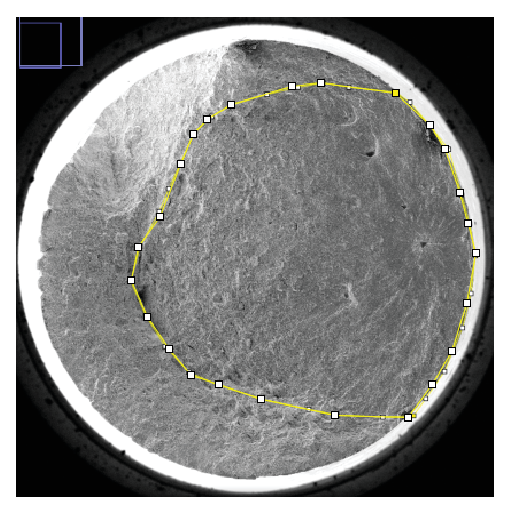
\includegraphics[width=3in]{P1MF19.eps}
  \caption{The crack in model P1MF19 marked with a yellow polygon.}
  \label{fig:P1MF19}
   \end{center}
\end{figure*}
%
The crack was marked manually.
The crack area is 11.118~mm$^2$ and the size of the ligament is $A_{\mbox{uncracked area}}=8.12$~mm$^2$.
Using eq.~(\ref{eq:sig_net}) and noting $\sigma_0=634$~MPa,
                           $\sigma_{net}=1502$~MPa.
The value found is much higher than the allowed stress $\sigma_f=1092$~MPa [how to cite Carmel confidential work??].
This finding shows the need for automatic marking of the crack.


%
%
\textcolor{green}{Here continued the detail on the $\sigma_{net}$ AI model.}

%%%%%%%%%%%%%%%%%%%%%%%%%%%%%%%%%%%%%%%%%%%%%%%%

Next, an example of a calculation of $K$ is presented.
The calculation is conducted for specimen P1MF19.
In order to use equation~(\ref{eq:K_I__F_I}), the crack front is approximated as an ellipse, as shown in Fig.~\ref{fig:P1MF19_elip_crack}.
%
\begin{figure*}[t!]
  \begin{center}
  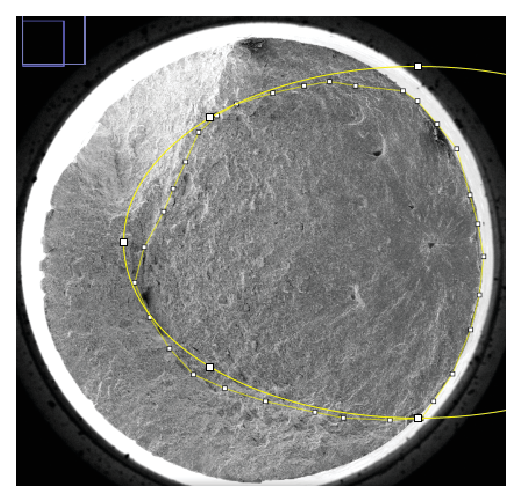
\includegraphics[width=3in]{P1MF19_elip_crack.eps}
  \caption{The crack in model P1MF19 marked with a yellow ellipse.}
  \label{fig:P1MF19_elip_crack}
   \end{center}
\end{figure*}
%
The ellipse was marked manually.
The values of $a, b$ and $D$ are 4.5~mm, 4~mm and 4.9~mm, respectively.
The range of the value $a/b$ in~\cite{shin2004experimental} is between 0 to 1.
Since here $a$ is larger than $b$, the aspect ratio between them is taken as 1.
The value of $F_I$ for $\frac{a}{b}=0, \frac{a}{D}=0.454$ and $\frac{x}{h}=0$, using eq.~(\ref{eq:F_I}), is ~1.042 (Need to be checked with the real equation. I took it from the table in~\cite{shin2004experimental}).
This is the value of $F_I$ at the middle of the crack front.
The value of $F_I$ for $\frac{a}{b}=0, \frac{a}{D}=0.454$ and $\frac{x}{h}=1$, using eq.~(\ref{eq:F_I}), is ~1.402 (kana"l).
This is the value of $F_I$ at the edges of the crack front.
Using eq.~(\ref{eq:K_I__F_I}) and noting $\sigma_0=634$~MPa, $K_I=56~\mbox{MPa}\sqrt{\mbox{m}}$ and $K_I=75\mbox{MPa}\sqrt{\mbox{m}}$ at the middle and at the edges of the crack front, respectively.
The value of the critical stress intensity factor, $K_{Ic}$, is $70~\mbox{MPa}\sqrt{\mbox{m}}$.
The value of $K_I$ at the middle of the crack front is much lower than the critical value.
The value of $K_I$ at the edges of the crack front is similar to the critical value.
It seems that the reason of the failure is due to the large $\sigma_{net}$ presented in Section~\ref{Subsec: Flow stress calculation model}.
The large value of $K_{Ic}$ at the edges of the crack front is unreasonable.
If the value was indeed such large, the crack should have propagated to the edges and not at the middle of the crack front.



\section{Conclusions and Future Work}
\label{Sec: Conclusions and future work}

\subsection{Conclusions}
This study demonstrated the effective adaptation of the U-Net architecture for the segmentation of external and internal contours in scanning electron microscope (SEM) images, significantly enhancing both the accuracy and efficiency of material analysis. Through the integration of sophisticated neural network techniques, specifically tailored for the complexities of SEM data, the customized U-Net model has shown robust capabilities in detailed feature extraction and precise image segmentation.

A key innovation in this approach was the implementation of heatmaps for internal contour detection. These heatmaps have proven indispensable in identifying and localizing fracture zones within materials, providing a high level of detail that facilitates in-depth analysis of material behavior and failure mechanisms. Additionally, the development of automatic calculation methods utilizing these heatmaps has markedly improved the speed and reliability of analyses, reducing dependence on labor-intensive manual methods and enhancing the objectivity of the results (Section~\ref{Subsubsec: Heatmap Evaluation}).

As demonstrated in Section~\ref{Subsec: Hypothesis Validation}, the U-Net model achieved high accuracy in detecting external and internal contours, with IOU values of 97.8\% and 87.6\%, respectively. Additionally, as mentioned in Section~\ref{Subsubsec: U-Net Model Application Evaluation}, the model successfully identified the internal and external contours of the fracture surfaces. This was confirmed through visual and quantitative comparisons with manual analyses, showcasing the model's effectiveness in detecting critical structural features.

The model also demonstrated notable performance in detecting contours in specimens from Selective Laser Melting (SLM) and Electron Beam Melting (EBM) processes, albeit with slightly lower accuracy compared to the primary analysis. These specimens were extracted from SEM images.

However, the model performed poorly for specimens extracted from other imaging modalities, such as Stereomicroscope.
Further research is needed to enhance the model's adaptability to diverse imaging techniques and materials, ensuring its broad applicability in material science research and industrial quality control.


\subsection{Advantages of Heatmap Use and Automated Calculations}
The introduction of heatmap techniques has transformed the process of SEM image analysis by providing a clear and intuitive visual representation of critical structural features within materials. These heatmaps enable analysts to focus their efforts more effectively, ensuring that potential issues are quickly identified and addressed. The automation of the segmentation process, built on this heatmap foundation, has brought several significant advantages:
\begin{itemize}
    \item \textbf{Reduced Need for Expert Analysis:} The automation significantly reduces the reliance on fractographic experts for initial image evaluations, allowing them to focus on complex analyses where human expertise adds the most value.
    \item \textbf{Increased Accuracy:} Automated tools minimize human error and provide a consistent standard for identifying and analyzing material defects.
    \item \textbf{Enhanced Efficiency:} The reduction in manual intervention speeds up the analysis process, allowing for quicker decision-making in research and development.
    \item \textbf{Standardization:} Automated calculations ensure that results are reproducible and comparable across different studies and settings, facilitating broader scientific validation.
\end{itemize}


\subsection{Potential Uses and Developments}

The methodologies developed in this study have broad applications in material science research and industrial quality control. The ability to accurately segment and analyze SEM images opens up new avenues for understanding material properties, failure mechanisms, and performance characteristics.

The automated calculation methods, based on the U-Net architecture and heatmap analysis, can be further refined and extended to address a wide range of material science challenges, including:

\begin{itemize}
    \item \textbf{Material Characterization:} The automated processes can be applied to a variety of materials, especially metals, to characterize their microstructures and fatigue failure modes under cyclic loads, and to calculate stress intensity factors, flow stresses, and other critical parameters.
    \item \textbf{Quality Control:} The automated analysis can be integrated into industrial quality control processes to detect defects, cracks, and other anomalies in manufactured components, ensuring product reliability and safety.
    \item \textbf{Failure Analysis:} The detailed fracture analysis enabled by the U-Net model and heatmap techniques can provide valuable insights into the root causes of material failures, guiding improvements in material design and manufacturing processes.
    \item \textbf{Research and Development:} The automated segmentation and analysis methods can accelerate research and development efforts by providing rapid and accurate feedback on material properties and performance, facilitating the design of new materials with enhanced characteristics.
\end{itemize}

These methods can be applied to various industries, including but not limited to:

\begin{itemize}
    \item \textbf{Aerospace:} Titanium alloys are widely used in aerospace applications due to their high strength-to-weight ratio and corrosion resistance. The ability to accurately analyze microstructural features and defects in these materials is crucial for ensuring the safety and reliability of aerospace components. Additive Manufacturing (AM) still has a long way to go before it can be used in critical aerospace applications. The ability to detect and analyze defects in AM parts is essential for ensuring their structural integrity and performance. Additionally, AM tends to result in relatively high porosity, which can lead to reduced mechanical properties and fatigue life. ~\cite{montanari2023additive}
    \item \textbf{Automotive:} The automotive industry has recently turned to the use of lightweight materials, such as titanium, to downsize components, improve fuel efficiency, and reduce emissions. AM is employed to reduce overall life cycle costs.~\cite{nyamekye2023impact}
    \item \textbf{Biomedical:} Titanium alloys have wide applications in the biomedical field, such as dental implants and joint replacements. A weak point of Selective Laser Melting (SLM) is the presence of residual stresses, which have a significant impact on the mechanical properties of the material. These patterns of stresses are significant when producing trauma devices, where the material is subjected to high loads.~\cite{marin2023biomedical}
\end{itemize}

\subsection{Future Work}
\textcolor{green}{Building on the successes of this project, future research directions are prioritized based on their potential impact and feasibility. Each direction aims to enhance the robustness, applicability, and efficiency of our methodologies in SEM image analysis.}

\begin{itemize}
    \item \textbf{Algorithm Enhancement:} Future work will focus on enhancing noise reduction techniques and improving edge detection. Enhanced noise reduction will make the algorithms more robust against varying SEM image qualities, while advanced edge detection will improve the accuracy of contour segmentation, particularly in complex microstructures. These refinements are crucial for ensuring reliable segmentation across diverse SEM conditions, thereby enhancing the overall effectiveness of the model.

    \item \textbf{Material Diversity:} Expanding the model’s application to include a broader range of materials and conditions is essential for verifying its adaptability and effectiveness in diverse scientific fields. Future work will focus on making the model more robust to different resolutions and different materials, ensuring consistent performance across varied datasets. Additionally, the model’s adaptability to images from different imaging techniques, not just SEM, will be explored to enhance its versatility. Hypotheses for future exploration include testing the model on composites, metals, and polymers to assess its ability to detect material-specific features and provide detailed insights into structural integrity and failure mechanisms.

    \item \textbf{Real-time Analysis Capabilities:} Developing real-time processing features is a promising direction for dynamic testing environments where immediate results can significantly enhance workflow efficiency. Preliminary steps include optimizing the computational efficiency of the U-Net model and employing hardware accelerations like GPUs and TPUs. Real-time capabilities will be particularly impactful in applications such as in-situ monitoring and quality control, where rapid feedback is essential.

    \item \textbf{User-Friendly Software Development:} Developing user-friendly software interfaces for non-experts to utilize the model in industrial and research settings is crucial. These interfaces will make advanced image analysis accessible to a broader audience, facilitating wider adoption and application of the methodologies developed in this study.

\end{itemize}

The methodologies developed and refined in this study hold great promise for transforming material science research. As these techniques evolve, their impact on the field is expected to grow, leading to more efficient material design processes and more effective failure analysis.





%% The Appendices part is started with the command \appendix;
%% appendix sections are then done as normal sections
%% \appendix




%\begin{thebibliography}{00}


 \bibliographystyle{elsarticle-num}
 \bibliography{bibs}




%\end{thebibliography}
\end{document}
\endinput
%%
%% End of file `elsarticle-template-num.tex'.
